
%%
%% This file contains examples of slides
%% that contain:
%%  1) an itemized list
%%  2) an enumerated list
%%  3) mathematical equations
%%  4) source code
%%
%% Edit this file in Linux by
%% typing:
%%   emacs slides-template.tex &
%%
%% Create slides to use in your presentation. 
%% Follow the examples that I have given you.
%%
%% Create a PDF file from this file
%% by typing:
%%   pdflatex slides-template.tex
%%
%% Display a PDF file in Linux by
%% typing:
%%   evince slides-template.pdf &
%%

\documentclass{beamer}
\title{Difference between FCFS and Short job first schedualing}
\author{Nam Phan}
\institute{Cornell College}
\date{04 December 2015}

\usepackage{graphicx}
\usepackage{hyperref}
\usepackage{amsmath}
\usepackage{listings}
\usepackage{adjustbox}
\lstset{language=c}

\setlength{\parskip}{12pt}

\usetheme{Warsaw}

%% Try any of these themes:
%% AnnArbor
%% Antibes
%% Bergen
%% Berkeley
%% Berlin
%% Boadilla
%% CambridgeUS
%% Copenhagen
%% Darmstadt
%% Dresden
%% Frankfurt
%% Goettingen
%% Hannover
%% Ilmenau
%% JuanLesPins
%% Luebeck
%% Madrid
%% Malmoe
%% Marburg
%% Montpelier
%% PaloAlto
%% Pittsburgh
%% Rochester
%% Singapore
%% Szeged
%% Warsaw

\usecolortheme{beaver}

%% Try any of these color themes:
%% albatross
%% beaver
%% beetle
%% crane
%% dolphin
%% dove
%% fly 
%% lily
%% orchid
%% rose
%% seagull
%% seahorse
%% whale
%% wolverine

\usefonttheme{default}

%% Try any of these font themes:
%% default
%% professionalfonts
%% serif
%% structurebold
%% structureitalicserif
%% structuresmallcapsserif

\begin{document}

\begin{frame}
  \titlepage
\end{frame}

\begin{frame}{Purpose}
\begin{center}
  Does short job first scheduler really improve the efficiency overall?
  \end{center}
\end{frame}

\begin{frame}[fragile]{Calculating statistic}
\begin{adjustbox}{width=\textwidth}
  \begin{lstlisting}{}
   void computeStuff( QueuePointer qp ) {
   NodePointer np = qp->pointerToHead;
   while (np != NULL ) {
    ProcessPointer currentPp = np->processPointer;

    if (np->pointerToNextNode != NULL) {
      currentPp->arrivalTime = currentPp->interarrivalTime + 
                                np->pointerToNextNode->processPointer->arrivalTime;
      currentPp->serviceStartTime = fmaxf(currentPp->arrivalTime, 
      np->pointerToNextNode->processPointer->serviceCompleteTime);
    } else {
      currentPp->arrivalTime = currentPp->interarrivalTime;
      currentPp->serviceStartTime = currentPp->arrivalTime;
    }

    currentPp->serviceCompleteTime = currentPp->serviceStartTime 
                                              + currentPp->serviceTime;
    np = np->pointerToPrevNode;
  }
}
    \end{lstlisting}
\end{adjustbox}
\end{frame}


\begin{frame}[fragile]{Adding processes to queues} 
  \begin{lstlisting}
  QueuePointer beforeQp = buildQueue(5);;
  PriorityQueuePointer pqp = createPriorityQueue(5);
  computeStuff(beforeQp);
  
  QueuePointer afterQp = createQueue(); 
  while (!isPriorityQueueEmpty(pqp)) {
    ProcessPointer pp = pqDequeue(pqp);
    enqueue(afterQp,pp);
  }
  computeStuff(afterQp);
  \end{lstlisting}
\end{frame}

\begin{frame}{Results}
\begin{align*}
  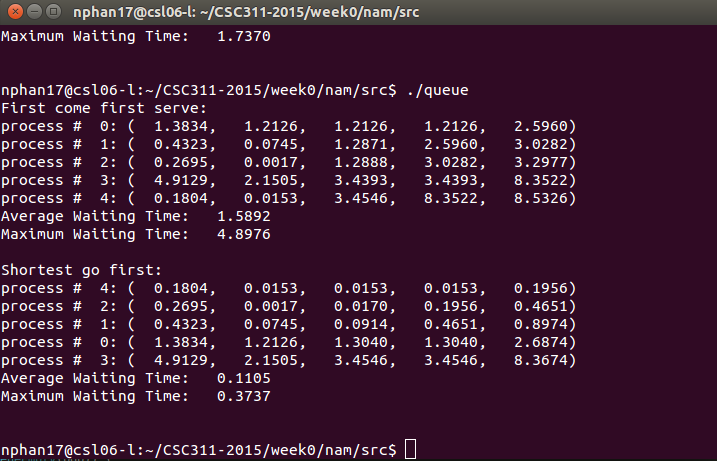
\includegraphics[width=\linewidth]{results}
  \end{align*}
\end{frame}

\begin{frame}{More Analysis}
\begin{align*}
  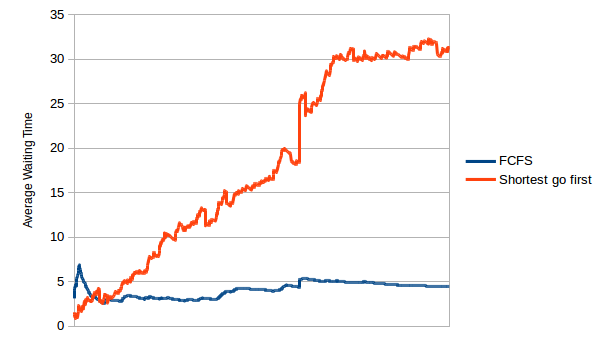
\includegraphics[width=\linewidth]{comparisonp};
\end{align*}
\end{frame}



\end{document}

